\chapter{Architecture}

\section{Bobox}

In the section we describe basic architecture of Bobox. Information source for this chapter is Doctoral thesis Parallel Processing of Data\cite{faltthesis}. 

Overall Bobox architecture is displayed in figure~\ref{fig:bobox}. Framework contains of Boxes. Box is basically a C++ class containing implementation of data processing algorithm or it can be set of connected boxes. Box can have arbitrary number of inputs and outputs. All boxes are connected to a directed acyclic graph.  

\begin{figure}[h!]
  \centering
    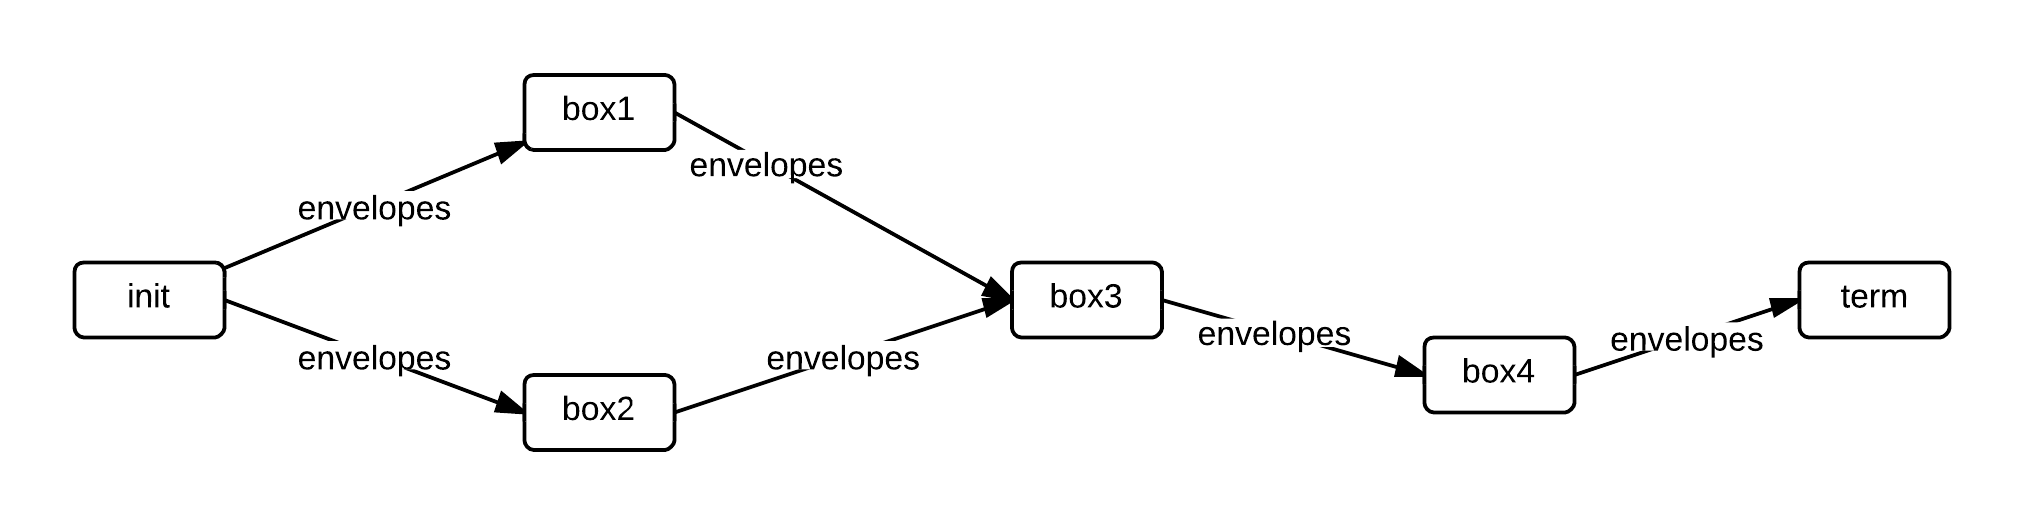
\includegraphics[width=1\textwidth]{bobox}

      \caption{Bobox architecture.}
          \label{fig:bobox}
\end{figure}

Data streams are implemented as data units called enveloped. Envelope structure is displayed in figure~\ref{fig:envelope}. It consists of sequence tuples, but internally data are stored by columns, that means envelope contains from sequence of columns and it's data is stored in separate list. So to read all attributes of the i-th tuple we have to access all column lists and read it's i-th element. There is special type of envelope having poisoned pill. It is send after all valid data indicating end of data stream. 

\begin{figure}[h!]
  \centering
    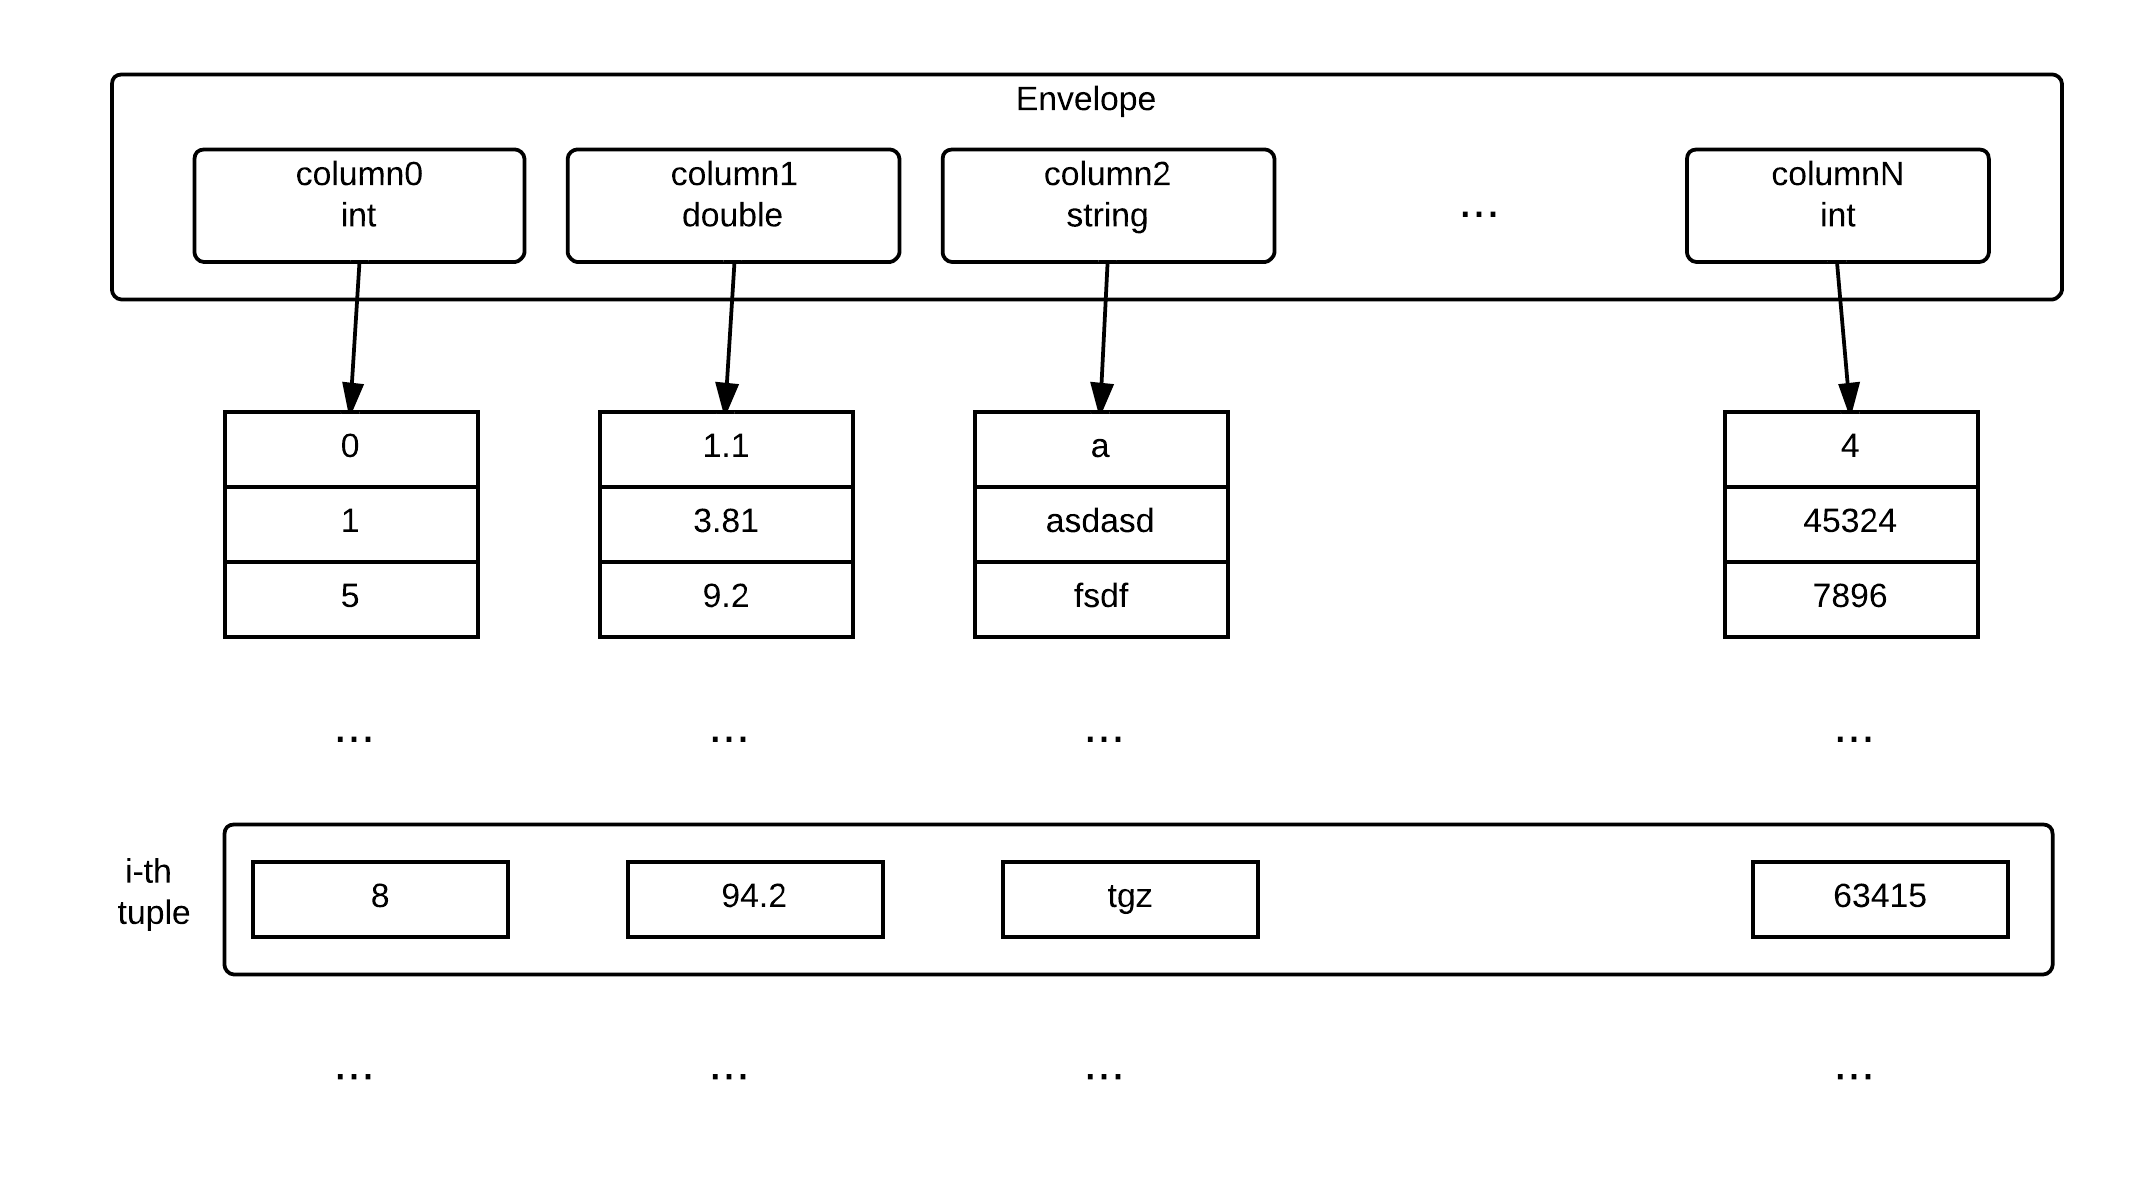
\includegraphics[width=1\textwidth]{envelope}

      \caption{Envelope structure.}
          \label{fig:envelope}
\end{figure}
There are two special boxes, which have to be in every execution plan:
\begin{itemize}


\item $init$ - first box in topological order and it indicates starting box of execution plan

\item $term$ - last box in topological order and indicates that plan has been completely evaluated

\end{itemize}

Evaluation starts with scheduling $init$ box, which sends poisoned pills to all of its output. All of it's output boxes will be scheduled. They can read data from hard drive or network, process it and sent it to other boxes for further processing. Other boxes usually receives data in envelopes in their inputs. Box $term$ waits for every it's input to receive poisoned pill and then evaluation ends.

\section{Bobolang}
In this section we describe syntax and semantics of Bololang language. We used paper Bobolang - a language for parallel streaming applications\cite{bobolang} as information source.

Bobolang is a formal description language for Bobox execution plan. Bobox environment provides implementation of basic operators (boxes). Bobolang let's programmer choose which boxes to used, what boxes to use, what type are passed and how the boxes are interconnected. Bobolang also provides possibility to create operators connecting existing ones. 

In following example we show a definition using other operators:

\begin{verbatim}
operator process (int)->(int,int,int)
{
    preproc(int)->(int,int) pre;
    post(int,int)->(int,int,int) post;
	
    input -> pre;
    pre -> post -> output;
}
\end{verbatim}

Code specifies that we are creating new operator called \verb|process|. It takes one stream of integers as input and outputs one stream of triplets integers. 

In the first part we declare sub operators, define type of input and output. For every declared sub operator we provide identifier. Second part specifies connection between declared operators. Code \verb|op1 -> op2| indicates that output of \verb|op1| is connected to input of operator \verb|op2|. In this case output type of \verb|op1| has equal to input type of \verb|op2|. Bobolang syntax also allows to create chains of operators like \verb|op1 -> op3| which has semantics like \verb|op1 -> op2| and \verb|op2 -> op3|. 

There are explicitly defined operators called \verb|input| and \verb|output|. They represents input and output of declared operator \verb|process|. The line \verb|input -> pre;| represents that input of the operator \verb|process| is connected to operator \verb|pre|.

Boblang also allows to declare operators with empty input or output. They have type \verb|()| that means it doesn't transfer any data. Only data allowed is to transfer poisoned pill. When box receives poisoned pill, it means that it should start working, Sending it means that it's work is done.

We can define whole execution plan using operator main with empty input and output. Example of whole Bobolang plan:

\begin{verbatim}
operator main()->()
{
    source()->(int) src;
    process(int)->(int,int,int) proc;
    sink(int,int,int)->() sink;

    input -> src -> proc -> sink -> output;
}
\end{verbatim}
 In figure~\ref{fig:exampleplan} we can seen structure of example execution plan. Operators \verb|init| and \verb|term| are added automatically. Operator \verb|init| sends poisoned pill to \verb|source|, which can read data from hard drive or network. These data are send to box \verb|process|. Operator sink stores data and sends poisoned pill to box \verb|term| and the computation ends.
\begin{figure}[h!]
  \centering

    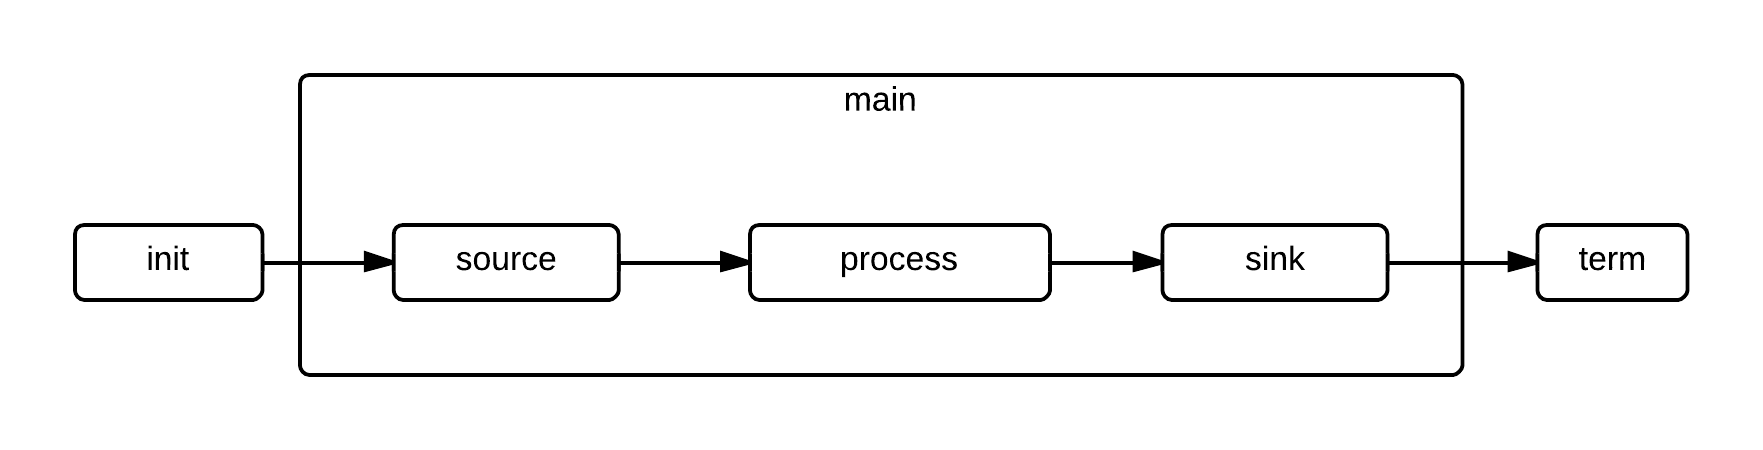
\includegraphics[width=1\textwidth]{exampleplan}
    
      \caption{Example of execution plan.}
        \label{fig:exampleplan}
\end{figure}


\section{SQL compiler architecture}
In this section we describe planed SQL compiler. It's architecture is displayed in figure~\ref{fig:sqlarchitecture}. 
\begin{figure}[h!]
  \centering

    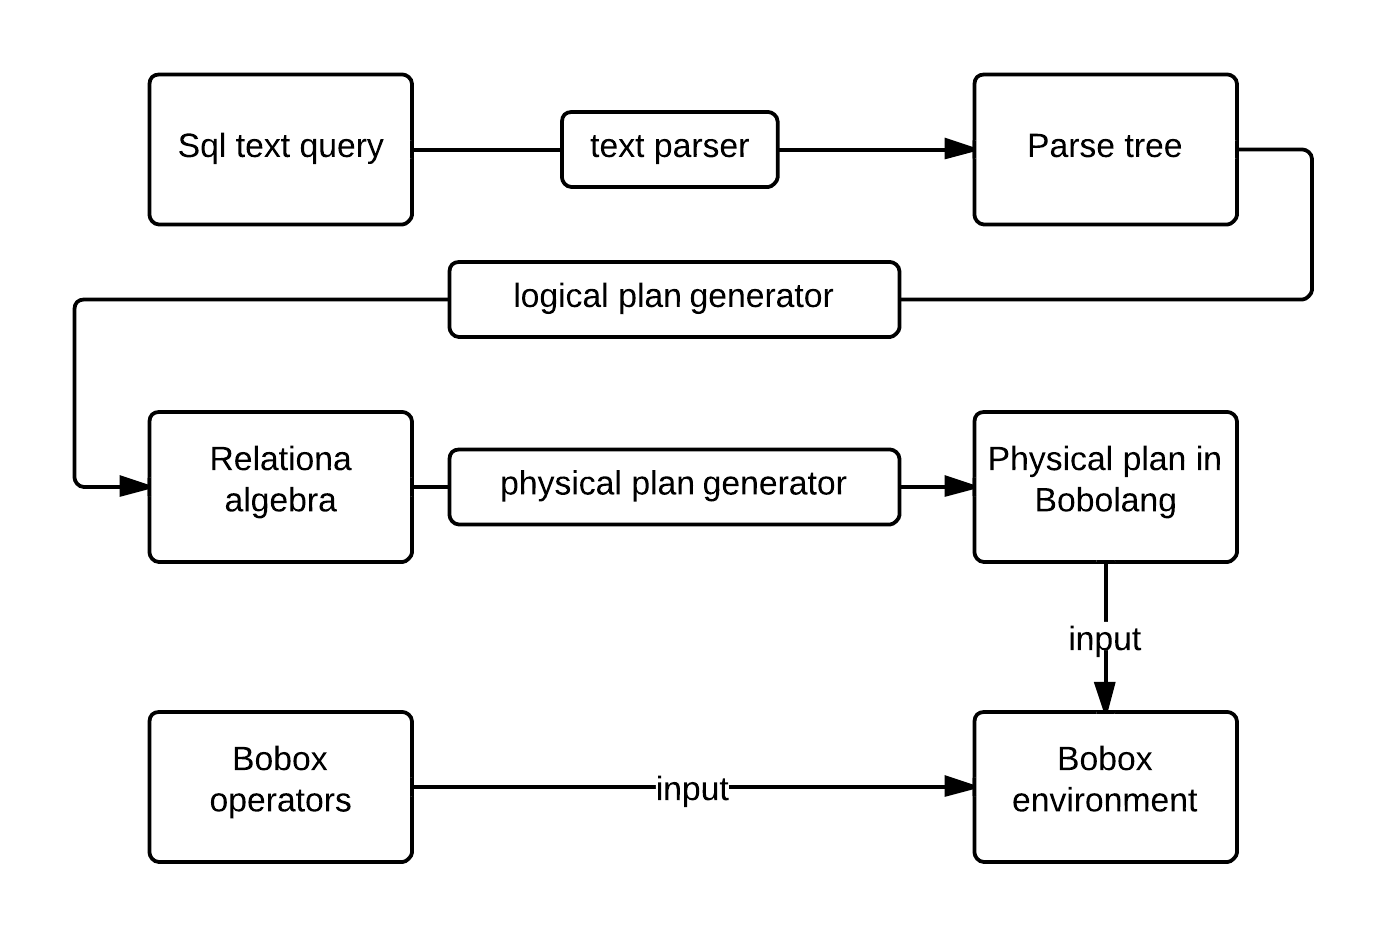
\includegraphics[width=1\textwidth]{sqlarchitecture}
    
      \caption{SQL compiler architecture.}
        \label{fig:sqlarchitecture}
\end{figure}

SQL query is written in text. This text is parsed into parse tree, which is transformed into logical query plan (Relational algebra). Relational algebra is then optimized and this form is used for generating physical query plan. Physical plan written in Bobolang is input for Bobox for execution. Physical plan is not enough, we need to also provide implementation of physical algorithms (Bobox operators).

Since SQL is a pretty complicated language, this thesis aim is only implementing optimization and transformation of logical plan into physical plan.


